% 
%qt-dab
%
\documentclass[12pt]{article}
\usepackage[pdftex]{graphicx}
\usepackage{amssymb}
\usepackage{latexsym}
\usepackage{relsize}
\usepackage{textcomp}
%processed for 10 pt 
%\documentstyle[epsf,psfig]{article}
%\documentstyle[epsf]{article}
\oddsidemargin 0pt
\topmargin -0.0cm
\textwidth 6.2in
\textheight 8.5in
\baselineskip 18pt
%\renewcommand{\baselinestretch} {1.5}
\newenvironment{nitemize}
   {\begin{list}{\begin{math}\bullet\end{math}}%
      {\setlength{\leftmargin}{5mm}
       \setlength{\topsep}{1mm}
       \setlength{\parsep}{0in}
       \setlength{\itemsep}{.7mm}}}%
   {\end{list}}

\newcommand{\fract}[2]{\frac{\textstyle #1}{\textstyle #2}}
\newcommand{\trans}[3]{#1 \stackrel{#2}{\longrightarrow} #3}
\newcommand{\notrans}[3]{#1 \stackrel{#2}{\not\! \longrightarrow} #3}
\bibliographystyle{plain}
\addtocontents{toc}{\setcounter{tocdepth}{2}}
\begin{document}
\title{Qt-DAB Users Guide
\ \\
{\it{\small  Open Source DAB Decoders}}
}
\author{
Jan van Katwijk\footnote{J.vanKatwijk at gmail dot com}, 
Lazy Chair Computing \\
The Netherlands}

%\date{}
\maketitle
%\baselineskip 22pt
\ \\
\begin{center}
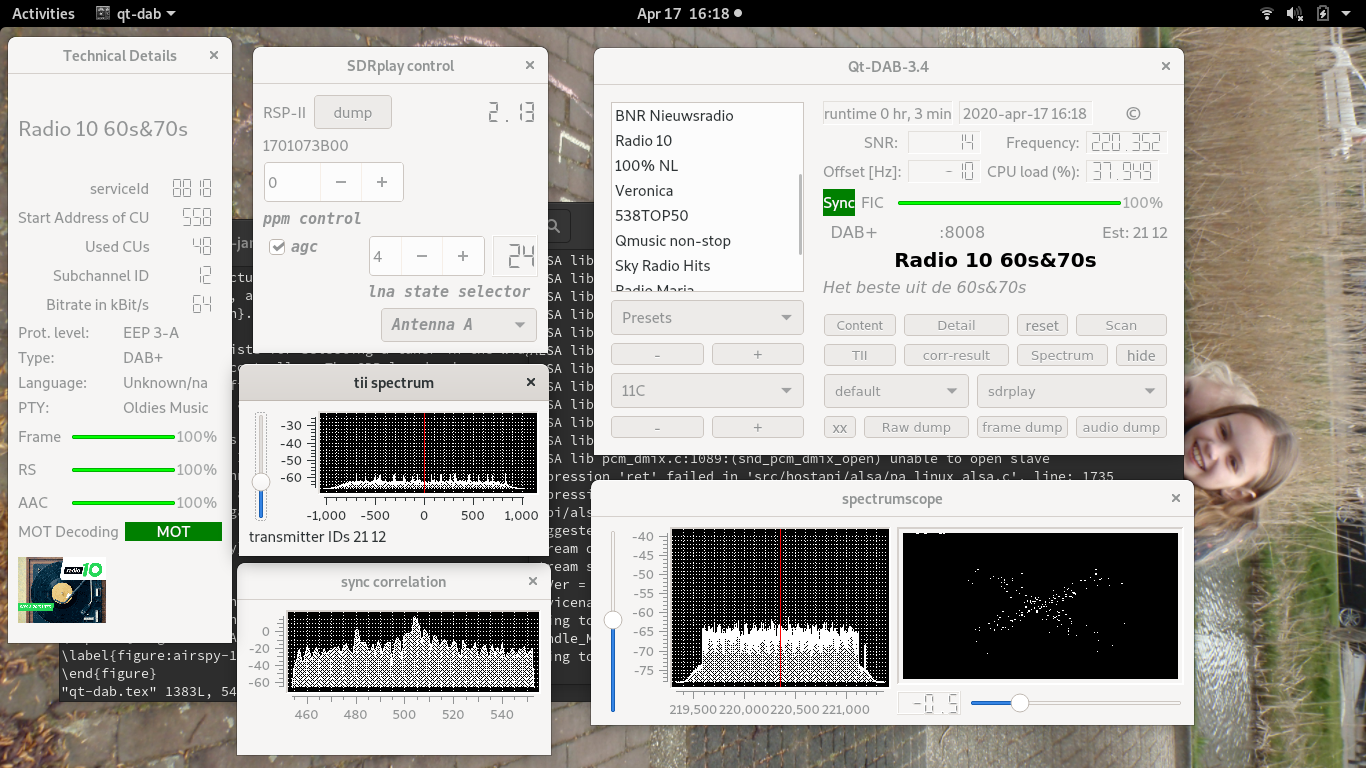
\includegraphics[width=160mm]{qt-dab-1.png}
\end{center}
\newpage
\tableofcontents
\newpage
\section{Introduction}
Qt-DAB is a program for decoding terrestrial DAB transmissions.
The program is implemented in C++, with extensive use
of Qt for its graphical appearance. Furthermore, it uses a number of existing
open source libraries and Qt-DAB is itself open source.
\par
Qt-DAB is designed to run on both Linux (x64) computers, including
RPI 2 and up, and is cross compiled for Windows.
\par
For {\em Linux (x64)} a so-called {\em appImage} is available,
a kind of container,
an executable file that contains next to the executable program
the libraries needed to run.
For {\em Windows} two {\em installers} are available, one
for the 32 bit version and one for the 64 bit version.
The installer will install the executable together with the required libraries.
These precompiled versions can be found in the releases section of the
repository for Qt-DAB (https://github.com/JvanKatwijk/qt-dab/releases).
\par
For RPI's, no preconfigured, precompiled
executable is available. This document contains a
pretty detailed description on how to build such an executable.
\par
The sourcetree for Qt-DAB contains - obviously - sources to generate
an executable for Qt-DAB. It actually contains subdirectories for {\em three}
decoder versions (next to a number of shared subdirectories),
{\em dab-maxi}, {\em dab-mini} and {\em dab-2}.
\begin{itemize}
\item {\em dab-maxi} contains sources specific to the Qt-DAB program,
the configuration files (i.e. a ".pro" file and a "CMakeLists.txt" file)
and the files needed for having an appImage for Qt-DAB when uploaded to
git (through Travis).
\item {\em dab-mini} contains sources, with configuration files and with
a description on how to create an executable version with a minimal interface.
\item {\em dab-2} contains sources for an experimental version,
a version with - roughly - the same functionality as Qt-DAB, however with
a completely different front end architecture.
\end{itemize}
This {\em dabMini} version is described is section 7 and for {\em Windows}
an installer is available.
\par
Since no {\em major} changes\footnote{Most likely there will be many
minor changes though.} to the Qt-DAB sources are expected, it
was considered time to do some user documentation.
\par
The structure of this guide is simple, in section 2 the GUI and GUI
widgets for the Qt-DAB program are discussed, in section 3
command line parameters and the settings in the ini file,
for the Qt-DAB program are discussed,
in section 4 the supported devices and their control widgets
for the Qt-DAB program are briefly discussed.
\par
In section 5, a description is given on how to build an
executable from the Qt-DAB and shared sources.
First the configuration parameters are briefly discussed,
a  description is given of  which libraries have to be
installed on a Linux system,
and what to do with either cmake or qmake.
\par
In section 6 the {\em device interface} as used in Qt-DAB
is discussed and an explanation is given how to interface a device
to the system configuration (note that the device interfaces for {\em dabMini}
and {\em dab-2} are different.
\par
Finally in section 7, a brief description is given of the {\em dabMini}
program,
a decoder version built on the same set of sources but with a minimal
interface.
\section{The GUI and GUI elements}
When playing around with DAB I am usually interested in properties
of the signal, and I want to be in control.
The GUI of Qt-DAB reflects this, there is an abundant amount of buttons,
selectors and displays.
\par
To keep things manageable, the GUI is built up as a central widget, a widget
that is shown permanently, together with a number of other widgets that might -
or might not - be made visible, depending on user's settings.
\par
While the figure on the first page shows the GUI with all
widgets,  figure \ref{figure:main-widget} shows the central widget, the
one with (most of) the controls.
\begin{figure}[htp]
\centering
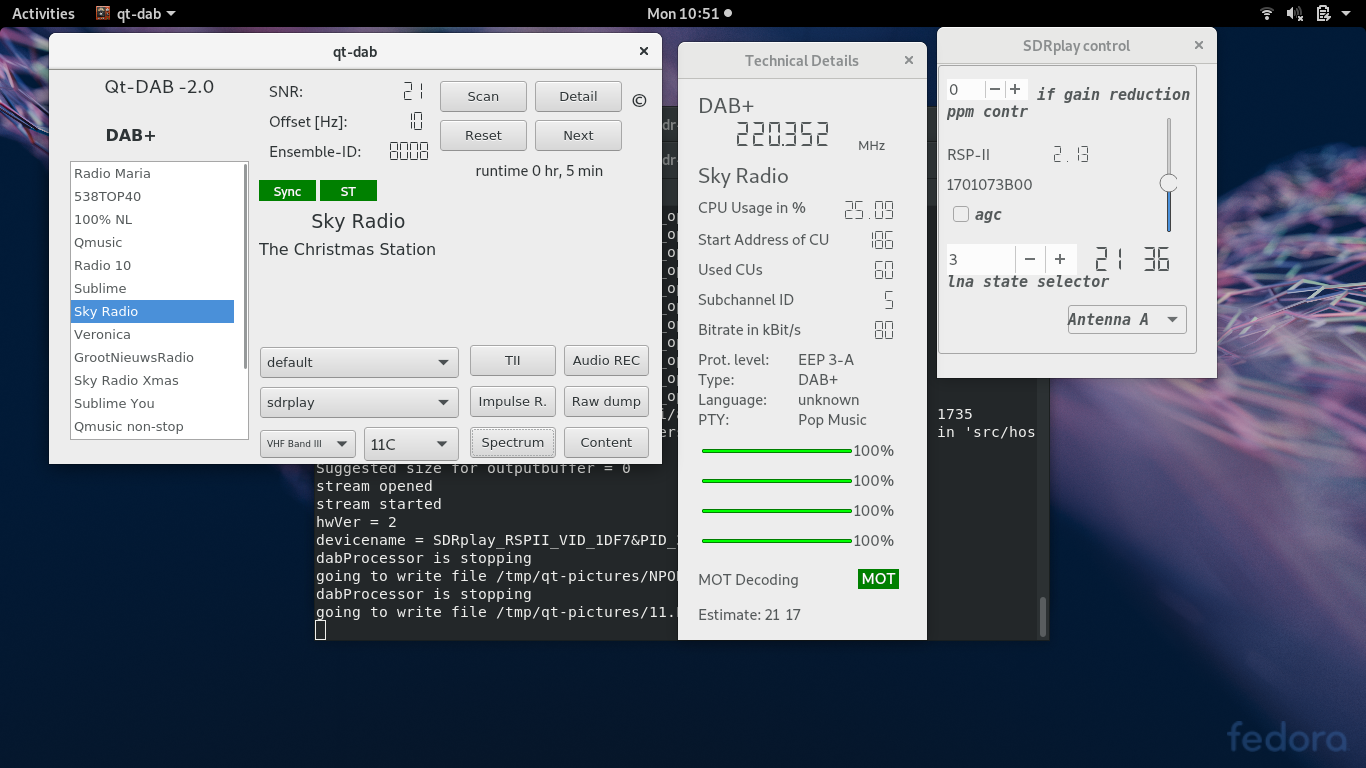
\includegraphics[width=100mm]{qt-dab-2.png}
\caption{Qt-DAB: the main widget of the GUI}
\label{figure:main-widget}
\end{figure}
\par
This main widget can be thought to consist of three elements:
\begin{itemize}
\item the left part, handling control for channel and service;
\item the top right part displaying information;
\item the bottom right part, the various controls.
\end{itemize}
Note that controlling an input device is using a  separate, device specific
control widget.
\subsection{Control for channel and service}
\begin{figure}[htp]
\centering
\includegraphics[width=30mm]{qt-dab-21.png}
\caption{Qt-DAB, channel and service selection}
\label{figure:left-part}
\end{figure}

Central in the left part of the GUI is the list of services, the list shows
the services detected in the currently selected channel.
{\em Selecting} a service is by moving the curson to the name of
a service, and clicking with the {\em left} mouse button.
\par
Below the list of services (see figure \ref{figure:left-part})
there is (from top to bottom)
\begin{itemize}
\item the combobox for the {\em presets}. A preset can be {\em added}
to this list by clicking with the {\em right} mouse button on the name of
the selected service in the service list\footnote{Clicking with the
right mouse button on the name of a service that is {\em not} the
selected one, will cause a small widget to be shown with
some information on the service pointed to}. Clicking with the left
mouse button on the entry in the preset list instructs the software
to select the {\em channel}, wait until the services of the channel
are visible, and finally, select the service.
{\em Removing} an element from the list is
by putting the cursor on the name of the service in the list of presets,
and pressing the {\em shift} and {\em delete} button on the keyboard
simultaneously.
\item a {\em previous} ($-$) and a {\em next} ($+$) service button.
With these button one can easily scan through the list of services.
\item the combobox for {\em channel selection}.
While DAB transmissions are in Band III, configuration provides
options to select channels in the {\em L Band}
or channels in a user defined band.
\item a {\em previous} ($-$) and a {\em next} ($+$) channel button,
making it easy to scan through the channels in the selected band.
\end{itemize}
Note that the software will "remember" which channel was selected, and
which service was selected. On (regular) program termination
these values will be saved, and on program start up, these values will
be taken as start value.
\par
Note furthermore that, starting with Qt-DAB-3.5, the software will "remember"
the gain settings for each channel and, on selection of that channel - either
explicitly or implicitly through selecting a preset service - restore
the gain setting as it was\footnote{A setting in the ini file exists to
ignore previous settings}.
\subsection{Displaying information}
\begin{figure}[htp]
\centering
\includegraphics[width=80mm]{qt-dab-22.png}
\caption{Qt-DAB, system wide information}
\label{figure:system-wide}
\end{figure}

Some general information is displayed in the top half of
the right side of the GUI, see figure \ref{figure:system-wide}.
The top line gives three elements
\begin{itemize}
\item the {\em run time}, the amount of time the program is running;
\item the {\em current time}, this time is taken from the time
encoding in the transmission. When playing a recording, the time found
in the recording is shown rather than the current time of listening;
\item the {\em copyright symbol}. Touching this with the cursor will reveal (a.o)
the time and date the executable was built.
\end{itemize}
Below this line, there are boxes with labels:
\begin{itemize}
\item SNR, the measured signal/noise ratio. SNR is computed by comparing
the signal strength in the null period of the DAB frame to
the average strength during transmission of the datablocks in the DAB frame;
\item Frequency, the frequency, in MHz, of the selected channel;
\item Offset, the frequency correction to be applied to the signal;
\item CPU load, the overall CPU load, i.e. not only for running the program.
\end{itemize}
\par
Below these - system related - pieces, there is a line with 
\begin{itemize}
\item the {\em sync} flag, if {\em green}, time synchronization is OK;
\item a {\em progressbar}, indicating the quality of
decoding of the data in the FIC (Fast Information Channel).
Since the FIC is "easier" to decode than
most of the other data, a value less than 100 percent here usually indicates
a poor reception.
\end{itemize}
\par
The remaining part of the widget is devoted to describing
the content of the reception,
the name of the ensemble is displayed together with its ID.
The name of the selected service is shown and below that name, the additional
text, i.e. the {\em dynamic label} is shown.
\par
The two numbers preceded by "Est:" give - if shown -
an estimate of the transmitter identification being received.
DAB is transmitted
using a {\em Single Frequency Network}, a network of transmitters, all
transmitting the same DAB content on the same frequency,
so one might (probaably will) receive data from more
than one of the transmitters at the same times and the software will
select the strongest signal.
Each transmitter in the network encodes a unique identification in
the transmitted signal,
the Transmitter Identification Information (TII), consisting of
two numbers, one to identify the network, one for the specific transmitter in that
network.
\subsection{Control elements}
\begin{figure}[htp]
\centering
\includegraphics[width=100mm]{qt-dab-23.png}
\caption{Qt-DAB: control elements}
\label{figure:control-elements}
\end{figure}

The controls are grouped in the lower right half of the GUI, displayed in
figure \ref{figure:control-elements}.
The control contains 12 push buttons and 2 comboboxes,
briefly discussed, in the order from left
to right, top to bottom.
\paragraph{Content button}
Touching the button labeled {\em Content} will instruct the software
to write a description of the content of the current ensemble to a file.
\begin{figure}[htp]
\centering
\includegraphics[width=120mm]{dab-content.png}
\caption{Qt-DAB: content}
\label{figure:content}
\end{figure}
First, a menu will be shown with which
the filename can be selected. The file is written in ASCII and is readable
by e.g. LibreOffice Calc or similar programs (see figure \ref{figure:content}).
\paragraph{Detail button}
Touching the button labeled {\em Detail} will instruct the software
to display detailed data on the selected service on a separate widget.
Touching the button again will hide the widget.

\begin{figure}[htp]
\centering
\includegraphics[width=35mm]{qt-dab-detail-button.png}
\caption{Service details}
\label{figure:service-details}
\end{figure}
\par
The widget - figure \ref{figure:service-details} -
shows the name and the identification of the service,
it shows where the data of the service is located in the input stream,
it shows the {\em protection} of the data against errors, whether it is
a DAB+ or a DAB transmission, and - if available -  it shows the
type of the service.
\par
New is the addition of a number that tells how many corrections on the
incoming DAB+ frames were needed (and could be performed). Note that
the maximum amount of errors that can be handled is 5 errors per frame.
Furthermore, a "stereo" indicator is back, now where it belongs, at the
description of the service.
\par
If the transmission of the service is also on FM, an FM frequency will be shown.
\par
For DAB+ services three progress 
bars are shown, in case all three
show a value of 100 percent, decoding is 100 percent. If less, then there
are some issues that could not be resolved
(the top one shows the successrate of DAB+ frames passing a first test,
the middle one the successrate of the Reed-Solomon error recovery on the
frames passing the first test,
and the bottom one tells the successrate of the AAC decoding).
\par
Below there progress indicators, a line will indicate whether or not
the service carries a MOT label. If it is, the picture
will be displayed.
The picture will be displayed by default on the widget for the detailed data,
however, a setting in the ".ini" file will cause the picture to be shown
on a separate widget.
\paragraph{Reset button}
Touching the button labeled {\em reset} will, as the name suggests, instruct the
software to do a reset on the selected channel,
i.e. synchronization will be done again and
a fresh list of services is built up - if any.
\paragraph{Scan button}
Touching the button labeled {\em Scan} will instruct the software to perform
a single scan over the channels in the currently selected band
(default Band III) and show the results, see
figure \ref{figure:scan-output} (i.e.
the names of the ensembles found, names of services and some technical data
on the services).
\begin{figure}[htp]
\centering
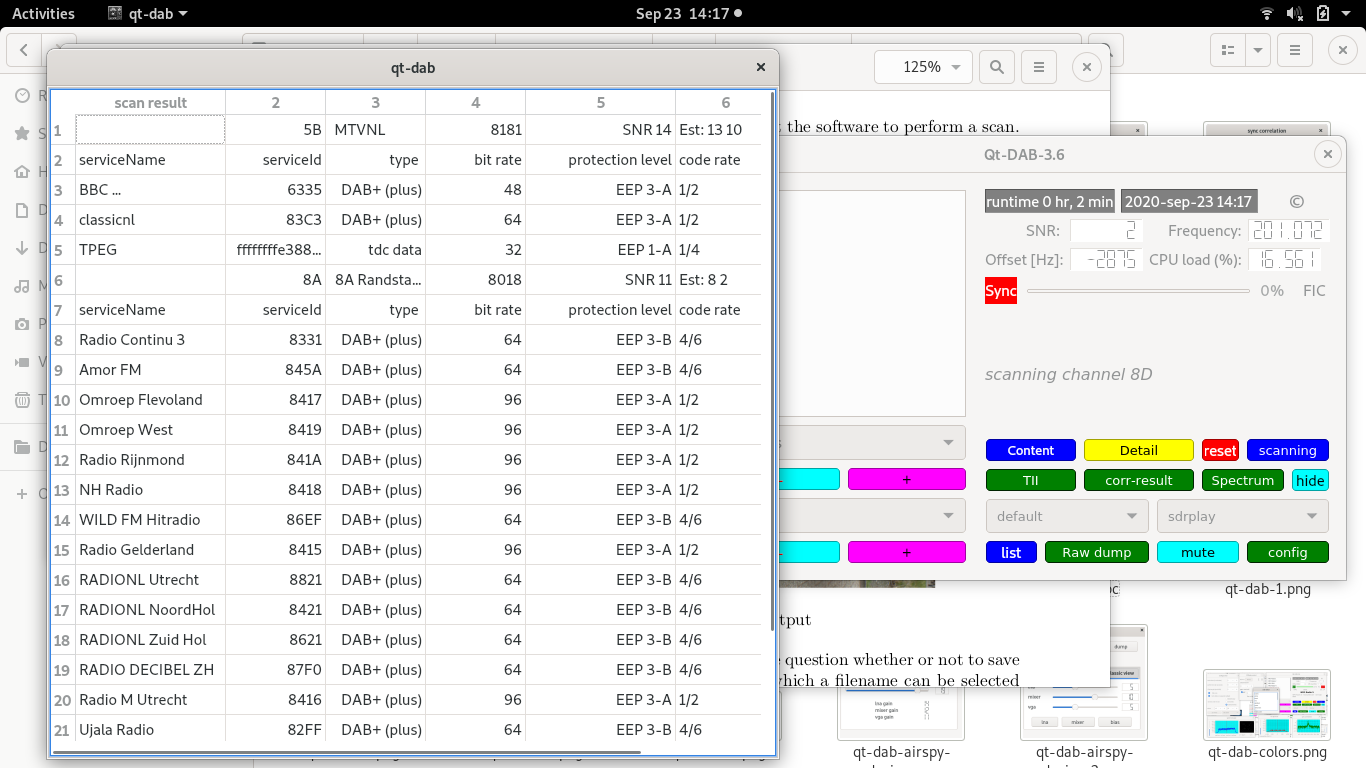
\includegraphics[width=120mm]{qt-dab-scan-button.png}
\caption{Fragment of the scan output}
\label{figure:scan-output}
\end{figure}
\par
Starting with Qt-DAB-3.5, a widget will be shown with the question whether
or not to save the result. If saving is selected, a menu will be shown
with which a filename can be selected (a suggestion for a filename,
containing the date and time is given). The result will then be saved
in a text file, that can be processed by e.g. LibreOffice Calc.
The format of the saved data is the same as the format of the data
saved when touching the content button, and the text shown is a subset of that.
\paragraph{TII button}
Touching the button labeled {\em TII} will instruct the software to
display a widget (figure \ref{figure:tii-spectrum}) with the
spectrum of the null period from the start of the DAB frames.
The TII data (Transmitter Identification Information)
is extracted from the spectrum of these null periods.
On touching the button again
the widget will disappear.
\begin{figure}
\centering
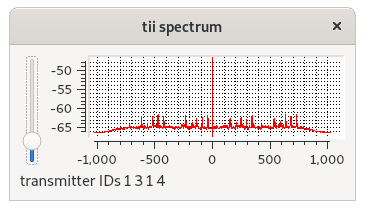
\includegraphics[width=60mm]{qt-dab-tii-button.png}
\caption{TII spectrum}
\label{figure:tii-spectrum}
\end{figure}
\paragraph{corr-result button}
Touching the button labeled {\em corr-result} will instruct
the software to display a separate widget, making
the {\em correlation result} for time synchronization visible.
As mentioned earlier,
DAB is transmitted in a Single Frequency Network and a receiver may
receive data from more than one transmitter. The signal from
the transmitter with the strongest signal (i.e. the highest correlation
value) is the  one used for demodulation and decoding.
\par
The X-axis indicates the sample numbers.
The picture, figure \ref{figure:correlation-result}, shows that there
are two peaks in the displayed region, one around sample 465 and one
near sample 505 (note that the default setting shows the correlation
over the first 1000 samples of a DAB frame, the width can be set in the ".ini"
file).
The latter is slightly stronger.
Given that the samplerate is 2048000, one can conclude that
the strongest signal arrives app 20 microseconds after the other one.
\par
Touching the button again will cause the widget to disappear.
\begin{figure}[htp]
\centering
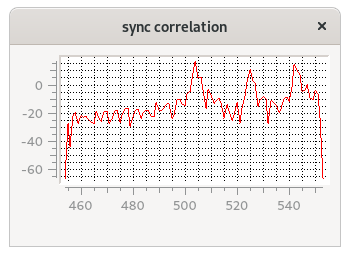
\includegraphics[width=60mm]{qt-dab-correlation-button.png}
\caption{Correlation result}
\label{figure:correlation-result}
\end{figure}

\paragraph{Spectrum button}
Touching the button labeled {\em Spectrum} will instruct
the software to display a separate widget, showing
the spectrum of the incoming signal, showing the constellation of the
received and decoded signal and showing a measure of the quality of the
signal.
The picture, figure \ref{figure:spectrum} shows a reasonable
though not excellent signal.
Ideally the constellation shows as four dots,
one in each quadrant. The more the constellation looks like a
collection of clouds,
the poorer the signal.

\begin{figure}[htp]
\centering
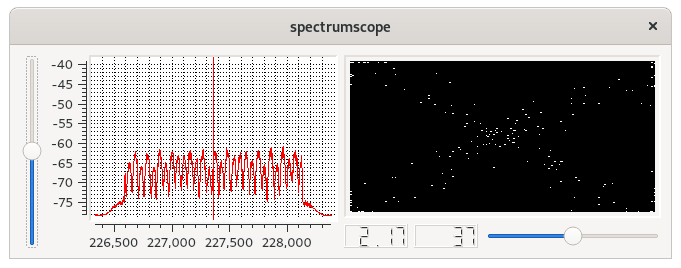
\includegraphics[width=100mm]{qt-dab-spectrum-button.png}
\caption{Spectrum of the signal}
\label{figure:spectrum}
\end{figure}

Below the constellation window, two numbers are shown.
The {\em quality indicator} shows - according to some metrics - the quality
of the constellation in a range from 0 .. 5. The {\em clock error} tells
the amount of samples too many or too few in processing 10 DAB frames
(a DAB frame is built up from 196608 samples with a rate of 2048000, so
10 DAB frames take slightly less than one second).
\par
As with the other buttons, touching the button again will cause the
widget to disappear.
\paragraph{hide button}
Touching the button labeled {\em hide} will hide
(or show) the widget for the 
device control. The text on the button shows what the action
following touching is (i.e. {\em hide} or {\em show}).

\paragraph{The combobox labeled {\em default}}
The combobox, labeled {\em default} in the picture is for selecting
an audio channel. What the combobox shows depends on the computer
where the program is running. In most cases {\em default} will do.
\paragraph{The combobox, labeled {\em sdrplay}}
The combobox labeled {\em sdrplay} in the picture is for selecting
a device. Depending on the configuration of the software device names will
show here.
\paragraph{xx button}
The  button labeled {\em xx} instructs the software to list the elements
in the {\em history file}.
Inspired by my car radio a list is
maintained of all services ever selected. Touching the {\em xx} button
again will hide the list (touching the list with the right mouse button
will clear it).
\paragraph{Raw dump button}
Touching the button labeled {\em Raw dump} will instruct the
software to dump the raw input samples into a file.
First, a menu is presented for selecting a filename. The menu will suggest
a filename of the form  "{\em device name}-{\em channel}-{\em date}.sdr" (date as derived
from the DAB stream).
Touching the button again will stop dumping and the file will be closed.
The resulting file is in PCM format, with a rate of 2048000, 2 channels and 
data represented as short ints.
Note that recorded files will be pretty large, per second more than
8 MByte is written.
\paragraph{frame dump button}
Touching the button labeled {\em frame dump} will  instruct the
software to write the AAC output of the selected
DAB+ service  to a file.
First, a menu is presented for selecting a filename. The menu will
suggest a filename of the form "{\em service name}-{\em date}.aac" (date  
as derived from the DAB stream).
Touching the button again will close the file.
The resulting file can be used as input to e.g.
VLC for further decoding.
\paragraph{audio dump button} 
Touching the button labeled {\em audio dump} will instruct the
software to write the audio output of
the currently selected service, to a file.
First a menu is presented for selecting a filename. The menu will suggest
a filename of the form "{\em service name}-{\em date}.wav" (date
as derived from the DAB stream).
Touching the button again will close the file.
The file, a PCM
formatted file, is written with samplerate 48000, 2 channels and 
short int (16 bits) format.
\section{Command line parameters and the ini file}
While the GUI provides lots of control, some settings can be done
via the command line or by setting values in the ".ini" file.
This ".ini" file also contains settings recorded by the software.
Its default name and location is {\em .qt-dab.ini} and it is kept in the
users home directory.
\subsection{Command line parameters}
On starting Qt-DAB via the command line (a few) parameters can be
passed:
\begin{itemize}
\item "-i filename" to use the file {\em filename} as ".ini" file rather than
the default one ".qt-dab.ini" which is stored in the users home directory;
\item "-P portnumber" to use the portnumber as port for {\em TPEG}
output in the Transparent Data Channel (tdc), which is - obviously
only meaningfull when configured.
\item "-A filename" to use the (name, integer) pairs in the file as channel definitions rather than the channels in Band IIIs. The sourcetree contains a
small file  as example: {\em testband}.
\item "-T" generate messages while processing on success and misses in the various decoding steps.
\end{itemize}
\subsection{Settings in the ".ini" file}
A number of settings can be done in the ".ini" file.
Note that, next to settings made by the user, the software
will store {\em some} settings on current 
selections (e.g, device, channel, service) in the ".ini" file.
\begin{itemize}
\item save\_gainSettings.
By {\em default} the gain settings per channel are saved in the ".ini" file.
Since these settings depend on the device, for each device section a
setting "save\_gainSettings=0" can be added to ignore previous values
for gain setting of that channel when selecting a channel.
\item dabMode:
While the {\em default} Mode for DAB is Mode 1, Qt-DAB provides the
possibility to use Mode 2 or 4 as well by setting "dabMode=X" (X in \{1, 2, 4\});
\item dabBand:
While the {\em default} DAB band is Band III,
Qt-DAB  provides the possibility
to use the L Band by setting "dabBand=L\_Band". Note that setting a value
here overrides the band setting by using command line parameters;
\item displaycolor:
While the {\em default} setting for the background color of the various
displays is {\em black}, setting "displaycolor=xxx" will set the
background of these displays to the selected color (e.g. "white");
\item gridcolor:
While the {\em default} setting for the color of the grids and the brushes
in the various displays is {\em white}, setting "gridcolor=xxx" will
set both the gridcolor as the color of the brush to the selected color (e.g.
"red");
\item displaySize:
While the {\em default} setting of the size of the X axis of the spectrum
and the TII display is 1024, setting "displaySize=xxx" will set the
size of the X axis to xxx, provided xxx is a power of 2;
\item plotLength:
While the {\em default} setting of the size of the segment to be seen
in the correlation viewer is 1000 (i.e. the correlation is shown
over the first 1000 samples of the datablock), setting "plotLength=xxx"
will show the correlation result over only xxx samples (centered around
the maximum correlation value);
\item saveSlides:
While the {\em default} is 1, implying that decoded slides are saved, setting
"saveSlides=0" will prevent slides to be saved;
\item motSlides:
While the {\em default} is 0, implying that decoder slides are displayed
on the {\em Technical data} widget, setting "motSlides=1" will cause
slides to be shown on a separate widget.
\item pictures:
While the {\em default} path for storing slides and pictures is the directory
"qt-pictures" in the /tmp directory, setting "pictures=xxx" will
use the folder "xxx" for that purpose.
\item epgPath:
While the {\em default} value is the empty string, implying that
files generated by the epg handler are not saved, setting "epgPath=XXX"
will use the "XXX" (if not the empty string) as path to these files
(assuming the path exists and the epg handler is configured in).
\item filePath:
While the {\em default} value is the empty string, implying that MOT files
other than slides and epg files, are not saved, setting "filePath=XXX"
will use "XXX" (if not the empty string) as path to these files
(assuming the path exists).
\item serviceOrder:
While the {\em default} order to display the services in the list of services
is alphabetically, setting "serviceOrder=1" will cause the services
to be displayed based on the order of their serviceIds;
\item normalScan:
While the {\em default} way a scan is performed is as a single scan
over all channels in the band, at the end displaying the result,
setting "normalScan=1" will instruct the software to start scanning
at the currently selected channel and stop scanning
as soon as a channel is encountered with DAB data;
\item history:
While the {\em default} file for storing (and reading back) the history
elements is ".qt-history-xml" in the users home directory, setting
"history=xxx" will use the file here denoted as "xxx";
\item switchTime:
While the {\em default} maximum delay taken into account to
select a preset value is 8000 milliseconds,
setting "switchTime=xxx" will use "xxx" (if specified 
as number) instead;
\item latency:
While the {\em default} value for the latency, i.e. the delay in handling the
audio, and determining the size of the audio buffers, is 5, setting
"latency=xxx" will set the value to "xxx" (if specified as positive number);
\item ipAddress:
While the {\em default} ip address for sending datagrams to (obviously only
meaningful if configured) is "127.0.0.1:, setting
"ipAddress=XXX" will use "XXX" as
ip address (if properly specified);
\item port:
While the {\em default} port address for sending datagrams to (obviously only
meaningful if configured) is "8888", setting
"port=XXX" will use "XXX" (if specified as positive number);
\item threshold:
While the {\em default} value for the threshold is 3, another value
can be set by "threshold=XXX". The threshold is a value used in the
time synchronization. If the maximum correlation found is at least
{\em threshold} times the average correlation value,
the maximum is considered to be OK;
\item tii\_delay:
While the {\em default} value for the number of DAB frames that will be 
skipped before recomputing the TII value is 5 (basically to reduce
the computational load), another value can be chosen by setting
"tii\_delay=XXX";
\item tii\_depth:
While the {\em default} value for the tii\_depth (i.e. the number of
spectra used to extract the TII values) is "1", another value can
be chosen by setting "tii\_depth=XXX";
\item echo\_depth:
While the {\em default} value for the echo\_depth is 1 (i.e. the maximum
amount of alternative peaks in the correlation), another value can be
chosen by setting "echo\_depth=XXX";
\end{itemize}

\section{Supported input devices}
The current version of Qt-DAB supports a variety of input devices,
the SDRplay, the AIRspy, the hackrf, the limeSDR and RT2832 based
sticks. Furthermore, there is {\em experimental} support for Pluto,
support for  the rtl\_tcp server, for devices for which a {\em Soapy}
interface is defined, and for file input.
\par
Both the {\em appImage} and the {\em Windows installer} are
configured with (almost) the whole range of devices: SDRplay RSP (both 
the 2.13 and 3.06 library versions),
the AIRspy, the hackrf, the LimeSDR, the Pluto and - of course - the RT2832 based
dabsticks. 
\par
\subsection{The SDRplay RSP}
The Qt-DAB software supports all RSP's from SDRplay.
Qt-DAB provides two different device handlers for the RSP's, one
for devices using the 2.13 SDRplay interface library,
the other one supports devices using the 3.06 SDRplay interface library.

\begin{figure}[htp]
\centering
\includegraphics[width=50mm]{qt-dab-sdrplay-213.png}
\includegraphics[width=50mm]{qt-dab-sdrplay-306.png}
\caption{The two control widgets for the SDRplay}
\label{figure:sdrplay}
\end{figure}
\par
As figure \ref{figure:sdrplay} shows, the control widgets
for the two different versions resemble each other, their implementations
differ considerably though.
Both have spinboxes for setting the {\em if gain reduction}, the
{\em lna state} and a {\em ppm offset}.
\par
An optimal value for the {\em ppm offset} is to be determined experimentally,
the RSP II, as used here, is happy with a ppm offset 0, the oscillator
offset is almost zero in the region of Band III.
\par
The spinbox for the {\em if gain reduction} is programmed to support
the range of values between 20 and 59.
The range of values for the {\em lna state}
depends on the model of the RSP. The software will detect the model
and fill in the range accordingly.
\par
If the {\em agc} is selected, the {\em if gain reduction}
spinbox will be hidden, its value is then irrelevant.
\par
The RSP II has two (actually 3) slots for connecting an antenna. If
an RSP II is detected, a combobox will be made visible for
{\em antenna selection}.
\par
A similar combobox exists for selecting a tuner in the widget
for the 2.13 library controller. The SDRplay duo has
two tuners. If the software detects the duo, a combobox will be made
visible for selecting a tuner (Note that this feature is not tested).
\par
Finally, both versions of the control widget contain
 a {\em dump} button. If touched, the
raw input from the connected device will be stored in a so-called xml
formatted file. First a menu is shown for selecting a filename,
a suggestion for the name of the file {\em device name} - {\em date} is
given.
Touching the button again will stop dumping and the file
will be closed.
\subsection{The AIRSpy}
\begin{figure}[htp]
\centering
\includegraphics[width=60mm]{qt-dab-airspy-device-2.png}
\includegraphics[width=60mm]{qt-dab-airspy-device.png}
\caption{Widgets for AIRspy control}
\label{figure:airspy-1}
\end{figure}
The control widget for the AIRspy (figure \ref{figure:airspy-1}, left)
 contains three sliders and a push button.
The sliders are to control the lna gain, the mixer gain and the vga gain.
\par
To ease balancing the setting of the sliders, two combined settings
are included in the widget, selectable by the tab {\em sensitivity} and 
{\em linearity}. Figure \ref{figure:airspy-1} right side, shows
the setting at selecting the tab {\em sensitivity}.
\par
Touching the button labeled {\em dump} instructs the software to dump
the raw stream of samples into a file in the xml format (Note that
while processing DAB requires the samplerate to be 2048000, that rate
is not supported by the AIRspy, implying that the driver software has to
do some rate conversion. The xml file though will just contain the
samples on the rate before conversion).
\subsection{The hackrf}
\begin{figure}[htp]
\centering
\includegraphics[width=70mm]{qt-dab-hackrf-device.png}
\caption{Widget for hackrf control}
\label{figure:hackrf}
\end{figure}
The control widget for hackrf (figure \ref{figure:hackrf}) shows,
next to the Serial Number of the device, a few sliders, a few checkboxes,
a spinbox and a push button.
\begin{itemize}
\item the {\em sliders} are there for controlling the lna and vga gain,
the slider values are limited to the range of possible values;
\item The {\em Ant Enable} checkbox is for Antenna port Power control (not used in this controller);
\item The {\em Amp Enable} checkbox is - if enabled - for additional gain
on the antenna input;
\item the {\em ppm correction} spinbox can be set to correct the oscillator
(on 227 MHz, the Qt-DAB software reports an offset of somewhat over 3 KHz);
\item the {\em Dump} push button when pushed, starts dumping the raw input in
xml file format. Touching the button again will halt the dumping and
close the file.
\end{itemize}
\subsection{The LimeSDR}
\begin{figure}[htp]
\centering
\includegraphics[width=50mm]{qt-dab-limeSDR.png}
\caption{Widget for lime control}
\label{figure:limecontrol}
\end{figure}

On selecting the LimeSDR (if configured), a control widget for the LimeSDR
is shown (figure \ref{figure:limecontrol}).
The widget contains just three controls:
\begin{itemize}
\item {\em gain} control, with predefined values;
\item {\em antennas}, where {\em Auto} is usually the best choice;
\item {\em Dump}, if touched, the raw input from the connected device
will be written to a file in the so-called xml format.
\end{itemize}
\subsection{The RTLSDR stick}
On selecting the dabstick (i.e. RT2832 based devices) (if configured),
a control widget for the device appears (figure \ref{figure:rtlsdrcontrol}).
\begin{figure}[htp]
\centering
\includegraphics[width=50mm]{qt-dab-rtlsdr-device.png}
\caption{Widget for rtlsdr device}
\label{figure:rtlsdrcontrol}
\end{figure}

The widget contains just a few controls:
\begin{itemize}
\item a {\em spinbox} for setting the ppm. Note that on average the offset
of the oscillator with DABsticks is (much) larger than that with devices
like the SDRplay. The DAB software is able to correct frequencies
to up to app 35 KHz, for some sticks the frequency error was large and
correction using the ppm setting was required.
\item a {\em combobox} for setting the gain.
The support software for RT2832 based
devices generates a list of allowable gain settings, these settings
are stored in the combobox;
\item a {\em combobox} for setting the autogain on or off;
\item a {\em push button} that, when touched, will instruct the software to
dump the raw input in the aforementioned xml format. At first a menu
appears for selecting a file. Touching the button again will stop dumping
and close the file.
\end{itemize}
\subsection{The Pluto device}
When selecting {\em pluto}, a widget (figure \ref{figure:plutocontrol})
appears with a spinbox for selecting
the gain, and a checkbox for selecting the agc.
\begin{figure}[htp]
\centering
\includegraphics[width=50mm]{qt-dab-pluto-device.png}
\caption{Widget for pluto device}
\label{figure:plutocontrol}
\end{figure}
The widget contains furthermore two buttons:
\begin{itemize}
\item the {\em debug control} button, when activated, instructs the software
to show output on each step in the initialization process (note that the
setting of the debug button will be maintained between invocations);
\item the {\em dump} button will cause the original input - with a samplerate
of 2100000 samples per second\footnote{The smallest samplerate that pluto
gives is slightly larger than the required 2048000, 2100000 is chosen
since it is easy to handle} - to be stored in an xml file.
\end{itemize}
\subsection{Support for Soapy}
{\em Soapy} is a generic device interface, a kind of wrapper to provide
a common interface to a whole class of devices. 
Qt-DAB supports Soapy, and its use is tested with the Soapy interface
for the SDRplay.

\begin{figure}[htp]
\centering
\includegraphics[width=50mm]{qt-dab-soapy-device.png}
\caption{Widget for soapy}
\label{figure:soapycontrol}
\end{figure}

The widget for soapy control (see figure \ref{figure:soapycontrol}) 
when applied to the Soapy interface for the SDRplay contains the obvious
controls, similar to that of the regular control for the SDRplay.
\subsection{File input}
Qt-DAB supports both {\em writing} raw input files and {\em reading} them back.
Writing a file as PCM file is initiated bythe {\em Raw dump} button on the main GUI,
writing a file as xml file by the {\em dump} button on
the various device widgets.
Qt-DAB differentiates between  reading
\begin{itemize}
\item raw 8 bit files as generated by e.g. Osmocom software (usually
files with an extension ".raw" or ".iq");
\item PCM (i.e. ".wav") files, provided the data is 2 channels and
with a samplerate of 2048000, generated by Qt-DAB and with an extension ".sdr";
\item xml files. The xml file format was defined by Clemens Schmidt
(author of QIRX)
and me and aims at saving files in the original format, so to
allow easy exchange between different DAB decoder implementations.
In order to support proper decoding of the contents, the data in the
file is preceded by a detailed description in xml, hence the name xml file format.
\end{itemize}
\begin{figure}[htp]
\centering
\includegraphics[width=70mm]{qt-dab-sdrfiles.png}
\includegraphics[width=70mm]{qt-dab-rawfiles.png}
\caption{Widgets for file input}
\label{figure:fileinput}
\end{figure}

When selecting file input ".raw" or ".wav", a simple widget is shown
(figure \ref{figure:fileinput}),
with as indication the number of seconds the file is being played.

\par
Since processing an xml file implies some interpretation, the
widget (figure \ref{figure:xmlfiles}) for control
when reading an xml file is slightly more complex.
It contains - next to the progress in reading the data - a description
of the contents of the file.
So, the program that generated the file as well as the device used in that
program are displayed, the number of bits of the samples, as well
as the number of elements is displayed as is the samplerate of recording and
the frequency of the recording.
\begin{figure}[htp]
\centering
\includegraphics[width=50mm]{qt-dab-xmlfiles.png}
\caption{Widget for xml file input}
\label{figure:xmlfiles}
\end{figure}
\par
Touching the {\em cont} button will instruct the software to restart
reading at the beginning of the segment in the file after reaching the end.
\section{Configuring and building an executable}
\subsection{Introduction}
While for both Windows and Linux-x64 there are ready-made executables
for installing resp. executing the Qt-DAB program, there are situations
where one wants (or needs) to create its own version.
For e.g. use of the software on an RPI one has to create an executable,
for e.g. using the software with other or non-standard configured devices
one has to create an executable.
This section will describe the configuration options and the building process.
\subsection{What is there to configure?}
The Qt-DAB software can be built using either qmake or cmake generating
a Makefile.
The current {\em configuration file} for qmake, {\em qt-dab.pro}, has
more options for configuring than the configuration file for use with cmake,
{\em CMakeLists.txt}.
\par
QMake and CMake take a different approach, while the configuration options
for use with qmake requires some editing in the {\em qt-dab.pro} file,
selecting configuration options with cmake is ususally through command line
parameters.
\par
Note that the {\em qt-dab.pro} file contains a section {\em unix}
and a section {\em win} for Windows that contain settings specific
to the OS used.
The CMakeLists.txt file is only used for Linux-x64.

\subsubsection{Finding the right qwt library (qt-dab.pro only)}
It turns out that linking the qwt library sometimes gives problems.
While in Fedora based systems, specifying linkage is as below,
i.e. the {\em -lqwt-qt5} is the right one, in Debian based systems the
line {\em -lqwt} line should be chosen by commenting out the other one.
{\small
\begin{verbatim}
#correct this for the correct path to the qwt6 library on your system
#LIBS           += -lqwt
LIBS            += -lqwt-qt5
\end{verbatim}
}
\subsubsection{Console or not (qt-dab.pro only)}
{\small
\begin{verbatim}
# CONFIG += console
  CONFIG -= console
\end{verbatim}
}

While for tracing and debugging purposes it might be handy to see
all the (text) output generated during execution, for normal
use it is not.
Including or excluding  {\em console} in the configuration
determines whether or not a console is present when executing.

\subsubsection{Configurable common devices}
Configuring devices is simple, for devices as mentioned above
as well as for {\em rtl\_tcp} the {\em qt-dab.pro} file 
and the {\em CMakeLists.txt} contain a description.
File input (all versions, i.e. raw files, sdr files and xml files) is
standard configured in Qt-DAB executables,
changing this would imply significant changes to the sources.

\paragraph{Using the qt-dab.pro file}
For configuring devices in the {\em qt-dab.pro} file, comment out or
uncomment the line with the devicename.
\begin{verbatim}
  CONFIG	+= dabstick
  CONFIG	+= sdrplay-v2
  CONFIG	+= sdrplay-v3
  CONFIG	+= lime
  CONFIG	+= airspy
  CONFIG	+= hackrf
  CONFIG	+= pluto
  CONFIG	+= soapy
  CONFIG	+= rtl_tcp
\end{verbatim}

Note that for {\em soapy}, and for {\em limeSDR} there is no support
in generating a windows executable, due to the absence of a suitable dll.

\paragraph{Using the CMakeLists.txt file}

The CMakeLists.txt file contains support for
AIRspy, SDRplay, SDRplay\_V3, RTLSDR, Hackrf, pluto and LimeSDR.
Including a device in the configuration is by adding "-DXXX=ON"
to the command line, where XXX stands for the device name.
\subsubsection{Configuring SSE}
In the deconvolution of the data in the FIC blocks, use is made
of deconvolution code generated by the spiral code generator.
If the code is to run on an x86-64 based PC, some speed up can be
obtained by using the code generated for use with SSE instructions.
Of course, the compiler used in the building process
 has to support generating the right
instructions, as fas as known, the Mingw compiler, used for
generating the windows executable, does not.
\par
The qt-dab.pro file contains in the unix section
\begin{verbatim}
CONFIG	+= PC
#CONFIG	+= RPI
#CONFIG	+= NO_SSE
\end{verbatim}
\par
Selecting "CONFIG += PC" selects SSE instructions, and deselects threading
of backends - after all, a standard PC has more than sufficient power to
run the decoding in a single thread.
\par
Selecting "CONFIG += RPI" selects options suitable for having the software
run on an RPI.
\par
Selecting "CONFIG += NO\_SSE" is for e.g. Mingw cross compiler for Windows.
\par
When using cmake, pass "-DVITERBI\_SSE=ON" as command line parameter
for PC's.

\subsubsection{Configuring audio}
\begin{itemize}
\item 
When running the Qt-DAB program remotely, e.g. on an RPI near a decent
antenna, one might want to have the audio output sent through an IP port
(a simple listener is available).
\item
Maybe one wants to use the audio handler from Qt.
\item
The default setting is to use {\em portaudio} to send the PCM samples
to a selected channel of the soundcard.
\end{itemize}
The {\em Linux} configuration for the Qt-DAB program offers in the
qt-dab.pro file the possibility of configuring the audio output:
\begin{verbatim}
#if you want to listen remote, uncomment
#CONFIG         += tcp-streamer         # use for remote listening
#otherwise, if you want to use the default qt way of sound out
#CONFIG         += qt-audio
#comment both out if you just want to use the "normal" way
\end{verbatim}

If cmake is used, pass "-DTCP\_STREAMER=ON" as parameter for
configuring the software for remote listening,
use "-DQT\_AUDIO=ON" for qt audio, or {\em do not specify anything} for
using portaudio in the configuration.
\par
Note that the configuration for Windows is only for "portaudio".
\subsubsection{Configuring TPEG in the tdc}
Handling TPEG in the tdc is only partially supported. Interpretation of the
data is not part of the Qt-DAB software, however, the software can
be configured to extract the TPEG frames and send these to an IP port.
\par
In the qt-dab.pro file, we have
\begin{verbatim}
#very experimental, simple server for connecting to a tdc handler
CONFIG         += datastreamer
\end{verbatim}
\par
In cmake the parameter "-DDATA\_STREAMER=ON"
can be passed to include handling TPEG  as described in Qt-DAB.

\subsubsection{Configuring IP datastream (qt-dab.pro only)}
IP data can be extracted from the DAB stream and send out through
an IP port.

\begin{verbatim}
#to handle output of embedded an IP data stream, uncomment
CONFIG          += send_datagram
\end{verbatim}

Note that - if not specified in the ini file - defaults are used for
ip address and port.
\subsubsection{Selecting an AAC decoder}
By default the {\em faad} library is used to decode AAC and generate the
resulting PCM samples.
{\em It turns out that both Ubuntu 20 and Fedora 32 install - by default - 
the libfaad-2.9 which is not compatible with the DAB+ output.}
\par
The source tree contains - in the directory {\em specials}, the sources
for the libfaad-2.8 version. It is quite simple to create and install
an appropriate library.
\par
An {\em alternative} is to use the {\em fdk-aac} library to decode AAC
(contrary to the libfaad the fdk-aac library is able to handle newer
versions of the AAC format, these newer versions are not used in DAB (DAB+)).
\par
Selecting the library for the configuration is by commenting
out or uncommenting the appropriate line in the file
{\em qt-dab.pro} (of course, precisely one of the two should be uncommented).
\begin{verbatim}
  CONFIG    += faad
  #CONFIG   += fdk-aac
\end{verbatim}
(see the subsection for installing the libraries).
\subsubsection{Configuring for platforms}
Processing DAB (DAB+) requires quite some processing power. On
small computers like an RPI2, performing all processing on a single
CPU core overloads the core. 
\par
In order to allow smooth processing on multi core CPU's, an option
is implemented to partition the workload.
In order to partition processing, uncomment
{\small
\begin{verbatim}
   DEFINES += __THREADED_BACKEND
   DEFINES += __MSC_THREAD__
\end{verbatim}
}
in the {\em qt-dab.pro} file.
\par
In case cmake is used, edit the file CMakeLists.txt and comment out
or uncomment the line 
\begin{verbatim}
#add_definitions (-D__THREADED_BACKEND)  # uncomment for use for an RPI
#add_definitions (-D__MSC_THREAD__)  # uncomment for use for an RPI
\end{verbatim}

It is recommended to use 
\begin{verbatim}
CONFIG	+= PC
\end{verbatim}
in the qt-dab.pro file,
when targeting towards a standard x64 based PC running Linux, using this
will set the SSE and the threading.
\par
It is recommended to use
\begin{verbatim}
CONFIG	+= RPI
\end{verbatim}
in the qt-dab.pro file when targeting for an RPI, the threading will be
set and the NO\_SSE option is set.
\subsubsection{Configuring EPG processing}
By default MOT data with EPG data is not dealt with. The
Qt-DAB sourcetree contains software from other sources that can be
used to decode EPG and write the decoded data into a file in xml format.
\par
In order to configure the software to include the epg handling part
uncomment
{\small
\begin{verbatim}
CONFIG          += try-epg        
\end{verbatim}
}
in the {\em qt-dab.pro} file, 
or add
{\small
\begin{verbatim}
-DTRY_EPG=ON
\end{verbatim}
}
to the command line when using cmake.
\subsection{Preparing the build: loading libraries}
\subsubsection{Installing the libraries}
Prior to compiling, some libraries have to be available.
For Debian based systems (e.g. Ubuntu for PC and Stretch for the RPI) one
can load all required libraries with the script given below.
{\small
\begin{verbatim}
   sudo apt-get update
   sudo apt-get install git cmake
   sudo apt-get install qt5-qmake build-essential g++
   sudo apt-get install pkg-config
   sudo apt-get install libsndfile1-dev qt5-default
   sudo apt-get install libfftw3-dev portaudio19-dev 
   sudo apt-get install zlib1g-dev rtl-sdr
   sudo apt-get install libusb-1.0-0-dev mesa-common-dev
   sudo apt-get install libgl1-mesa-dev libqt5opengl5-dev
   sudo apt-get install libsamplerate0-dev libqwt-qt5-dev
   sudo apt-get install qtbase5-dev
\end{verbatim}
}

If {\em libfaad} is the selected aac decoder, install
\begin{verbatim}
   sudo apt-get install libfaad-dev 
\end{verbatim}
If {\em fdk-aac} is the selected aac decoder, install
\begin{verbatim}
	sudo apt-get install libfdk-aac-dev
\end{verbatim}

If {\em Pluto} is (one of) the device(s) to be included in the
configuration, install
\begin{verbatim}
   sudo apt-get install libiio-dev
\end{verbatim}
\subsubsection{Downloading of the sourcetree}
Since the script also loads {\em git},
the sourcetree for Qt-DAB (including the sources for dab-mini)
can be downloaded from the repository by
{\small
\begin{verbatim}
  git clone https://github.com/JvanKatwijk/qt-dab.git
\end{verbatim}
}
The command will create a directory {\em qt-dab}.
\subsubsection{Installing support for the RTLSDR stick}
It is advised - when using an RT2832 based "dab" stick - to create
the library for supporting the device
{\small
\begin{verbatim}
   git clone git://git.osmocom.org/rtl-sdr.git
   cd rtl-sdr/
   mkdir build
   cd build
   cmake ../ -DINSTALL_UDEV_RULES=ON -DDETACH_KERNEL_DRIVER=ON
   make
   sudo make install
   sudo ldconfig
   cd ..
   rm -rf build
   cd ..
\end{verbatim}
}

\subsubsection{Installing support for the AIRspy}
If one wants to use an AIRspy, a library can be created and installed by
{\small
\begin{verbatim}
   wget https://github.com/airspy/host/archive/master.zip
   unzip master.zip
   cd airspyone_host-master
   mkdir build
   cd build
   cmake ../ -DINSTALL_UDEV_RULES=ON
   make
   sudo make install
   sudo ldconfig
   cd ..
   rm -rf build
   cd ..
\end{verbatim}
}
\subsubsection{Installing support for SDRplay RSP}
If one wants to use an RSP from SDRplay, one has to load and install
the library from "www.SDRplay.com".

\subsubsection{Making the installed libraries visible}
The installation of these device handlers will install libraries
in the \begin{verbatim} /usr/local/lib \end{verbatim} directory. Note that the path to this
directory is NOT standard included in the search paths for the Linux loader.
To add this path to the searchpaths for the Linux loader, create a file
\begin{verbatim}
/etc/ld.so.conf.d/local.conf
\end{verbatim}
with as content
\begin{verbatim}
/usr/local/lib
\end{verbatim}
The change will be effective after executing a "sudo ldconfig" command.
\par
The installation of these device handlers will furthermore install some files
in the \begin{verbatim}/etc/udev/rules.d \end{verbatim} directory.
These files will ensure that a non-root 
user has access to the connected device(s).
\par
Note that in order for the change to be effective, the {\em udev} subsystem has
to be restarted. The easiest way is just to reboot the system.
\subsection{Finally: building an executable}
\subsubsection{Using cmake to build the executable}
After installing the required libraries, and after editing
the configuration (if required), compiling the sources and generating an
executable is simple.
\par
Using cmake, creating an executable with as devices the SDRplay, the
AIRspy, and the RTLSDR based dabsticks, the following script can be used:
{\small
\begin{verbatim}
   cd qt-dab/dab-maxi
   mkdir build
   cd build
   cmake .. -DSDRPLAY=ON -DAIRSPY=ON -DRTLSDR=ON ... -DRTL_TCP=ON
   make
\end{verbatim}
}
\par
The CMakeLists.txt file contains instructions to install the executable
in "/usr/local/bin".
{\small
\begin{verbatim}
   sudo make install
   cd ..
   cd ..
\end{verbatim}
}

\subsubsection{Using qmake to build the executable}
Assuming the file qt-dab.pro is edited, the same result can be
obtained by
{\small
\begin{verbatim}
   cd qt-dab/dab-maxi
   qmake
   make
\end{verbatim}
}
{\em In some Linux distributions replace  qmake by qmake-qt5!}
\par
The {\em qt-dab.pro} file contains in both the section for unix as for
windows a line telling where to put the executable
{\small
\begin{verbatim}
DESTDIR         = ./linux-bin
\end{verbatim}
}
By default in Linux the executable is placed in the
{\em ./linux-bin} director in the {\em qt-dab} directory.
\section{Adding support for a device}
Qt-DAB is an open source project. Anyone is invited to suggest
improvements, to improve the code and to add code for e.g. yet unsupported
devices.
\par
While Qt-DAB can be configured for a variety of devices (basically
the devices I have access to), there is obviously a multitude of other
devices that are worthwhile to be used with Qt-DAB.
\subsection{The Qt-DAB device interface}
The Qt-DAB software provides a simple, well-defined interface
to ease interfacing a different device.
\par
The interface is defined as
{\small
\begin{verbatim}
class	deviceHandler: public QObject {
public:
         deviceHandler 	(void);
virtual	~deviceHandler 	(void);
virtual	int32_t	getVFOFrequency	(void);
virtual	int32_t	defaultFrequency(void);
virtual	bool	restartReader	(int32_t);
virtual	void	stopReader	(void);
virtual	int32_t	getSamples	(std::complex<float> *, int32_t);
virtual	int32_t	Samples		(void);
virtual	void	resetBuffer	(void);
virtual	int16_t	bitDepth	(void);
virtual	void	show		();
virtual	void	hide		();
virtual	bool	isHidden	();
virtual	QString	deviceName ();
private:
	QFrame	*myFrame;
};
\end{verbatim}
}

A device handler for a - yet unknown - device should implement this
interface.
\par
A description of the interface elements follows
\begin{itemize}
\item {\em getVFOFrequency} returns the current oscillator frequency in Hz;
\item {\em defaultFrequency} returns a frequency in the range
of valid frequencies;
\item {\em restartReader} is supposed to start or restart the generation of
samples from the device. Note that while not specified explicitly
the assumed samplerate is 2048000, with  the samples filtered
with a bandwidth of 1536000 Hz.
The parameter - in Hz - indicates the frequency to be selected.
{\em restartReader} when already running has no effect.
\item {\em stopReader} will do the opposite of restartReader, collecting samples
will stop; {\em stopReader} when not running has no effect.
\item {\em getSamples} is the interface to the samples. The function should
provide a given amount of samples, the return value is the number of
samples actually read.
\item {\em Samples} tells the amount of samples available for reading. If the
Qt-DAB software needs samples, the function Samples is continuously called
(with the delay between the calls) until the required amount is available,
after which {\em getSamples} is called.
\item {\em resetBuffer} will clear all buffers. The function is called on change
of channel.
\item {\em bitDepth} tells the number of bits of the samples. The value is
used to scale the Y axis in the various scopes and to scale the input
values when dumping the input. 
\item {\em deviceName} returns a name for the device. This function is
used in the definition of a proposed filename for {\em Raw dump}s.
\item The GUI contains a button to hide (or show) the control widget for
the device. The implementation of the control for the device will
implement - provided the control has a widget - functions to {\em show}
and to {\em hide} the widget, and {\em isHidden}, to tell
the status (visible or not). Note that if the widget for {\em newDevice}
is based on {\em myFrame}, the {\em default} implementation for 
these function does not to be reimplemented.
\end{itemize}

\subsection{What is needed for another device}
Having an implementation for controlling the new device, the Qt-DAB software
has to know about the device handler, which requires a change to
the configuration file (here we take qt-dab.pro) and
the file radio.cpp, the main controller of the GUI.

\paragraph{Modification to the qt-dab.pro file}
Driver software for a new device, here called {\em newDevice}, should
implement a class {\em newDevice}, derived from the class {\em deviceHandler}.
\par
It is assumed that the header is in a file {\em new-device.h}, the
implementation in a file {\em new-device.cpp}, both stored in a directory
{\em new-device}.
\par
A name of the new device  e.g. {\em newDevice}
will be added to the list of devices, i.e.
{\small
\begin{verbatim}
   CONFIG	+= AIRSPY
...
   CONFIG	+= newDevice
\end{verbatim}
}
Next, somewhere in the qt-dab.pro file a section describing XXX should
be added, with as label the same name as used in the added line with CONFIG.
{\small
\begin{verbatim}
newDevice {
   DEFINES         += HAVE_NEWDEVICE
   INCLUDEPATH     += ./devices/new-device
   HEADERS         += ./devices/new-device/new-device.h \
                        .. add further includes to development files, if any
   SOURCES         += ./devices/new-device/new-device.cpp \
                        .. add further implementation files, if any
   FORMS           += ./devices/new-device/newdevice-widget.ui
   LIBS            += .. add here libraries to be included
}
\end{verbatim}
}

\paragraph{Modifications to radio.cpp}

The file "radio.cpp" needs to be modified in three places
\begin{itemize}
\item  In the list of includes add
{\small
\begin{verbatim}
#ifdef	HAVE_NEWDEVICE
#include	new-device.h
#endif
\end{verbatim}
}
\item The names of selectable devices are stored in a combobox.
{\small
\begin{verbatim}
#ifdef	HAVE_AIRSPY
	deviceSelector	-> addItem ("airspy");
#endif
....
#ifdef	HAVE_NEWDEVICE
	deviceSelector	-> addItem ("newDevice");
#endif
\end{verbatim}
}
\item If selected, the class implementing the device handler should
be instantiated,
{\small
\begin{verbatim}
#ifdef	HAVE_AIRSPY
	if (s == "airspy") {
	   try {
	      inputDevice	= new airspyHandler ....
	....
#endif
#ifdef  HAVE_NEWDEVICE__
        if (s == "newDevice") {
           try {
              inputDevice       = new newDevice (..parameters..);
              showButtons ();
           }
           catch (int e) {
              QMessageBox::warning (this, tr ("Warning"),
                                   tr ("newDevice not found\n"));
              return nullptr;
           }
        }
        else
#endif
\end{verbatim}
}
\end{itemize}
\subsection{Static or dynamic linking}
The approach taken in the implementations of the different device handlers
is to load the required functions for the device library. This allows the
generation of an executable - even if some device libraries are not installed.
\section{dabMini}
\subsection{Why a dabMini}
I often run DAB decoder(s) on an RPI2 or 3. Since these RPIs are headless,
control is from my laptop.
Sometimes I find the GUI of Qt-DAB too large, especially when my only concern
is to listen to the audio. In that case I do not need any of the push buttons
and the comboboxes on the main GUI widget, nor the additional widgets.
\par
While I was using {\em dabRadio} for that purpose (or {\em qml-dab})
for some time, I realised that most of the corrections and changes
as applied to the sources - quite many - for Qt-DAB were not applied to
the sources of these programs.
\par
So, in order to maintain consistency of sources between Qt-DAB and a
version with a small GUI I designed and implemented {\em dabMini}
by using the Qt-DAB sources. To ensure 
consistency, a subdirectory was made in the Qt-DAB sources containing
the (few) files special for use with this dabMini. Interesting is
that - next to changes to device handlers to accomodate for the demise
of the device control widgets - only 2 files needed to be changed.
\subsection{The GUI}
\begin{figure}[htp]
\centering
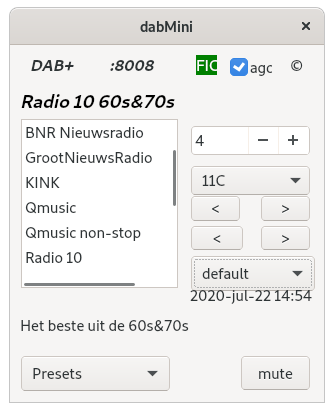
\includegraphics[width=70mm]{dab-mini.png}
\caption{dabMini}
\label{figure:dab-Mini}
\end{figure}
\par
As picture \ref{figure:dab-Mini} shows, the GUI is minimal.
The {\em device control} is at the top right. Depending on the
selected device, one or two spinboxes (usually some lna setting
and some other gain setting) are shown together with a checkbox
for the agc. {\em dabMini} will - on program start up - look for
any of the configured devices being connected, and take the
first one encountered.
\par
To the right of the service list, a {\em channel selector} is available,
with a $<$ (previous) and a $>$ (next) button for easy scanning though
the channels, and, below these,
 a $<$ (previous) and $>$ (next) button for easy
scanning though the services in the service list.
Below these buttons, there is the {\em audio channel} selector,
set by default on {\em default}.
\par
The bottom of the GUI contains the so-called {\em dynamic Label},
a large comboboxes labeled {\em Presets}, a stereo indicator
and a button labeled {\em mute}.

\paragraph{Presets}.
Presets are implemented as in Qt-DAB,
i.e. touching a {\em selected} service in the service list with the
right mouse button will add the "channel:name" pair describing the
service to the preset list. {\em Selecting} a preset service is
by touching the service in the service list with the {\em left} mouse button.
{\em Removing} a service from the preset list is
by putting the cursor on the name of the service in the list of presets,
and pressing the {\em shift} and {\em delete} button on the keyboard
simultaneously.
\paragraph{Stereo indicator}
Based on some user requests, a stereo indicator was re-introduced.
\paragraph{Mute}
Based on a user request, a {\em mute} button was added, the button - when touched - will mute the audio output for a number of seconds. Default value
is 10 seconds, the value can be changed by setting a value "muteDelay=xxx"
in the ini file, xxx indicates the number of seconds.
\par
Touching the mute button will sound is muted will end muting.
\subsection{dabMini on Windows}
While it is certainly possible to download the sources and build an
executable for windows, the {\em releases} section of the Qt-DAB
repository (https://github.com/JvanKatwijk/qt-dab/releases) contains
an installer for dabMini.
\subsection{dabMini on x64 Linux}
An appImage for dabMini, configured with the whole range of devices,
is available on the Qt-DAB repository.
\subsection{Building an executable on Linux and RPI}
As an example, loading libraries and building an executable of
the program on an RPI (running Buster) is described here.
\subsubsection{Installing the libraries}
For e.g. the RPI running Buster, the following lines
will install all required libraries
{\small
\begin{verbatim}
   sudo apt-get update
   sudo apt-get install git cmake
   sudo apt-get install qt5-qmake build-essential g++
   sudo apt-get install pkg-config
   sudo apt-get install libsndfile1-dev qt5-default
   sudo apt-get install libfftw3-dev portaudio19-dev 
   sudo apt-get install libfaad-dev zlib1g-dev rtl-sdr
   sudo apt-get install libusb-1.0-0-dev mesa-common-dev
   sudo apt-get install libgl1-mesa-dev libqt5opengl5-dev
   sudo apt-get install libsamplerate0-dev 
   sudo apt-get install qtbase5-dev
\end{verbatim}
}
\par
{\it Note that on other platforms libraries might be named in another way}.
\par
Assuming the only device that needs support is an RT2832 based stick,
execute the lines from the following script
{\small
\begin{verbatim}
   git clone git://git.osmocom.org/rtl-sdr.git
   cd rtl-sdr/
   mkdir build
   cd build
   cmake ../ -DINSTALL_UDEV_RULES=ON -DDETACH_KERNEL_DRIVER=ON
   make
   sudo make install
   sudo ldconfig
   cd ..
   rm -rf build
   cd ..
\end{verbatim}
}
Assuming support for Pluto is wanted, then install
\begin{verbatim}
	sudo apt-get install libiio-dev
\end{verbatim}
(see section 5.3.6 for some comments on making the device visible).
\par
\subsubsection{Download the sourcetree for Qt-DAB}
Dowload the sourcetree for Qt-DAB from the repository
{\small
\begin{verbatim}
  git clone https://github.com/JvanKatwijk/qt-dab.git
\end{verbatim}
}
\subsubsection{Generate an executable}
The settings in the file {\em CMakeLists.txt} are such that no changes
are needed, just execute the lines from the following script
(the "make" will take app 10 minutes on an RPI 3) to build and
install an executable.
{\small
\begin{verbatim}
   cd qt-dab
   cd dab-mini
   mkdir build
   cd build
   cmake .. -DRTLSDR=ON -DPLUTO=ON
   make
   sudo make install
   cd ..
   cd ..
\end{verbatim}
}

This will install the executable {\em dabMini-1.0} in {\em /usr/local/bin}.
\section{Acknowledgements}
Qt-DAB and derived programs are written and maintained by me.
The software is provided {\em as is}, and made available under the
Gnu GPL V2 license.
\par
Many people contributed
by providing feedback, suggestions and code fragments, in particular:
\begin{itemize}
\item Andreas Mikula for continuous feedback, testing and suggestions;
\item Stefan P\"oschel, for providing code for and giving suggestions to
handling the AAC code;
\item Stuart Langland for its comments, suggestions and code contributions;
\item probonopd for its contribution with creating appImages; and
\item Przemyslaw Wegrzyn for contributing code for handling
charsets.
\end{itemize}
Furthermore I am grateful 
\begin{itemize}
\item
to SDRplay ltd (Andy Carpenter) for providing me the possibility to use
different versions of the SDRplay RSP devices, all wonderful devices;
\item
to Benjamin Vernoux for making an AIRSPY device available;
\item to
Great Scott Gadgets for making an HACKRF device available;
\item
to Jan Willem Michels for making a LimeSDR device available, and
\item to Olaf Czogalla, for donating an RT2832 based stick after
having lively discussions on TPEG.
\end{itemize}
Qt-DAB is developed as hobby program in spare time.
Being retired I do have (some) spare time
and programming Qt-DAB (and my other programs) is just hobby.
Contributions are always welcome, especially contributions in the form of
feedback and additions and corrections to the code,
but obviously also in the form of equipment that can be used.
\par
If you consider a financial contribution, my suggestion is
to support the red cross or your local radio amateur club instead.
\end{document}

